\documentclass[a4paper,11pt]{report}
\usepackage[utf8]{inputenc}
\usepackage[T1]{fontenc}
\usepackage[francais]{babel}
\usepackage[top=2cm, bottom=2cm, left=2cm, right=2cm]{geometry}
\usepackage{graphicx}
\usepackage{geometry}
\usepackage{color}
\usepackage{fancyhdr}
\pagestyle{fancy}
\fancyhf{}
\lhead{2011/2012}
\rhead{IUT Nancy Charlemagne}
\geometry{hmargin=1cm,vmargin=2cm,lmargin=2cm,rmargin=2cm}
\lfoot{Licence ASRALL}
\cfoot{Rapport intemédiaire}
\rfoot{\thepage}
\renewcommand{\footrulewidth}{2pt}

% Title Page
\title{Archive, dé-duplication de données, compression : état de l'art, techniques et performances}
\author{Clément Ghnassia \\Mathieu Leroux \\Edgar Rodriguez}


\begin{document}

\maketitle
\tableofcontents

\chapter{Introduction}

\section{Analyse}

\paragraph{}
La sauvegarde est, de manière générale, une opération qui consiste à copier des données, souvent importantes, de façon à les protéger en cas de perte ou d'altérations de celles-ci ou des systèmes et supports sur lesquels elles sont stockées. 
Cette opération est assez proche de l'archivage. Même si les procédés mis en oeuvre sont les mêmes, l'objectif in fine est lui différent : 
tandis que la sauvegarde consiste à se prémunir contre d'évenutelles altérations de données encore utilisées, l'archivage consiste lui à conserver des données obsolètes dans un but plus historique, c'est à dire qui ne sont plus utilisées, mais dont on pourrait avoir besoin d'exploiter dans le futur.

\paragraph{}
Aujourd'hui plus que jamais, la sauvegarde des données est une opération critique pour les particuliers, mais encore plus pour les entreprises.
Bien qu'ils devraient avoir une place centrale et faire l'objet de toutes les attentions et de toutes les vérifications possibles, les processus de sauvegarde, et tout ce qu'ils englobent, sont souvent délaissés.
On explique assez facilement pourquoi tant de négligeances. 
Tout d'abord il faut comprendre que la sauvegarde n'est utilisée qu'en cas de pertes de données, ce qui est normalement rare dans une entreprise. 
Il n y a donc aucune visibilité pour les utilisateurs dans leur quotidien.
De plus, tous les moyens mis en oeuvre pour la sauvegarde impliquent des coûts qui ne seront jamais rentabilisés.
Il faut aussi avouer que la sauvegarde, malgré son importance, n'est pas ce qu'il y a de plus attrayant dans le domaine de l'informatique. 
Il est logique qu'elle ne soit pas aussi développée et normalisée que d'autres éléments dans le même domaine.

\paragraph{}
De nos jours, beaucoup d'entreprises n'utilisent exclusivement plus que l'informatique comme moyen de communication et pour le sockage de documents.
Des données critiques transitent donc sur le réseau et sont stockées dans des ordinateurs.
Il est donc vital pour l'entreprise de s'assurer que ces données ne seront pas perdues ou altérées en toutes circonstances.
C'est là que la sauvegarde, et tout ce que cela entraîne, prend toute son importance. 
A l'heure où le papier est de moins en moins utilisé, et ce au profit de l'informatique, il faudra veiller à ce que ces données soient protégées efficacement.
La sauvegarde est une des réponse à cet enjeu. De plus la sauvegarde implique la restauration et l'élaboration de plans de reprise d'activité.

\paragraph{}
On s'attachera donc à comprendre la sauvegarde, d'un point de vue méthodologie, puis pragmatique, avec les besoins nécessaires, l'importance dans le choix des stratégies, l'optimisation de ces procédés, et les bonnes pratiques à adopter.
Pour ce qui est de l`'optimisation des sauvegardes et des restaurations, on fera le tour des technologies existantes, expliquant les principes de fonctionnement de la compression et de la déduplication, ainsi que leurs intérêts dans un contexte de sauvegarde.
On verra aussi pourquoi elle doit évoluer de la même façon que l'informatique et les utilisations évoluent, comme le `` tout informatique `` ou encore l'augmentation d'ordinateurs portables dans les entreprises. 
Il s'agira donc de trouver des solutions adaptées ou des orientations à prendre.
On verra aussi comment les techniques de sauvegarde doivent s'adapter à l'infrastucture informatique déjà existante. 
Etant un point critique dans l'entreprise, et coûteux en terme d'investissement, il s'agira d'affiner au plus les stratégies de sauvegardes pour correspondre aux ressources et aux besoins.

\paragraph{}
Enfin, les données sauvegardées étant logiquement importantes, on s'attachera à protéger ces données aussi bien contre un évènement catastrophique, que contre un vol ou une exploitation de ces données.
On verra où et comment stocker ces données, et les techniques qui permettront de ne les rendre exploitables que par les utilisateurs qui sont habilités à le faire, comme le chiffrement par exemple.

\section{Problématique}

Un nombre considérable de questions et de réflexions sont générées lors de l'élaboration et la mise en place de sauvegardes, aussi bien à un niveau méthodologique que pratique.
Analyser ces différents aspects et pouvoir répondre aux questions permettront de trouver la solution ou la combinaison de solutions la plus adaptée en fonction du besoin.

\subsection{Objectifs}

L'aspect le plus important de la sauvegarde et le premier auquel on doit réfléchir est : quels sont les objectifs finaux de la sauvegarde ?
De quoi veut-on se prémunir. Quels sont les scénarios catastrophe auquels la stratégie de sauvegarde doit répondre ? 
Autant de questions primordiales et qui seront spécifiques à chaque situation.

\subsection{Contraintes}
Au delà des objectifs, il s'agira d'élaborer les contraintes, qui jouent aussi un rôle déterminant dans l'élaboration d'une stratégie de sauvegarde.
Si toutes les techniques de sauvegardes ne sont pas équivalentes en terme de sécurité et de performance, c'est aussi le cas au niveau des coûts.
L'élaboration d'une stratégie de sauvegarde qui devra se calquer sur une infrastructure déjà existante est souvent un réel investissement, et n'est pas à négliger.
Après les contraintes de coûts, il y a toutes les contraintes liées au contexte de sauvegardes, tel que la quantitée de données à sauvegarder, la fréquence des sauvegardes et la durée de rétention.

\subsection{Optimisation}
L'optimisation des sauvegardes est liées aux contraintes.
En effet, comme les contraintes sont bien présentes et sont un réel obstacle, il conviendra d'optimiser au maximum ces sauvegardes, aussi bien en termes de coûts que de performances et d'espace disque (qui sont liés).
Une partie sur l'optimisation sera développée et les technologies existantes seront présentées, tel que la compression et la déduplication.

\subsection{Données}
Cet aspect est lié aux objectifs et aux contraintes posés.
Il faudra savoir finement quelles données doivent être sauvegardées.
Sauvegarder des données inutiles engendrera un surcoût inutile, et ne pas sauvegarder des données importantes sera catastrophique lorsqu'on devra effectuer une restauration.
De plus, les données à sauvegarder sont évidentes lorsqu'il s'agit des données des utilisateurs, mais il faudra faire attention aux données relatives au système qui pourraient être critiques.
Une autre problématique liée au données et non négligeable est de pouvoir sauvegarder des données qui sont en cours d'utilisation et de modification. 

\subsection{Gestion}
On doit aussi de poser la question sur la gestion de la stratégie de sauvegarde au quotidien, comme l'automatisation des tâches et la supervision.
De plus en plus d'utilisateurs souhaitent aussi pouvoir effectuer eux même les opérations de sauvegarde et de restauration, sans avoir besoin d'avertir un administrateur.
Des techniques permettant la délégation des tâches qui les concernent seront explorées.

\subsection{Application}
Il s'agira d'effectuer un comparatif sur les différentes solutions existantes permettant de faire des sauvegardes, de manière plus ou moins automatisée.
En effet, un grand nombre de logiciels sont disponibles et avoir un comparatif permettrait de choisir la solution la plus adaptée.

\chapter{Etat de l'art}

\section{Sauvegarde}

Lors de l'élaboration d'une stratégie de sauvegarde, un très grand nombre de choix importants seront à faire, et cela à beaucoup de niveau.
Un grand nombre de possibilités existent chacun offrant des avantages par rapport aux autres.
Dans cette partie, nous allons explorer toutes les solutions existantes concernant les modèles d'entrepôts de données, les supports de sauvergarde et les gestions de dépots.

\subsection{Modèles}
Le modèle, c'est comment les données vont être organisées dans l'entrepôt de données, et donc de quelle manière les données seront sauvegardées. 
Il existe un nombre important de modèles, chacun offrant des avantages et des inconvénients.

\subsubsection{Non structurée}
Cette méthode consiste simplement à stocker des sauvegardes avec des informations sur la nature de ces sauvegardes et les dates auquelles elles ont été réalisées.

\subsubsection{Images du système}
Dans ce type de modèle, il s'agit de stocker une image complète du système à un instant donné.

\subsubsection{Différentielle}
Une sauvegarde différentielle consiste à sauvegarder uniquement les données qui ont été modifiées depuis la dernière sauvegarde complète.

\subsubsection{Incrémentale}
Une sauvegarde incrémentale consiste à sauvegarder uniquement les données qui ont été modifiées depuis la dernière sauvegarde, quelle qu'elle soit.

\subsubsection{Delta inversé}
Dans ce type de modèle, on aura un mirroir des données à leur état au moment de leur dernière sauvegarde.
On pourra revenir à un état antérieur grâce aux journaux de modifications sauvegardés.

\subsubsection{Protection des données en continu (CDP)}
Au lieu d'effectuer des sauvegardes périodiquement, les modifications sont envoyées instantanément vers l'espace de stockage dédié à la sauvegarde à travers le réseau.

\subsection{Dispositifs de stockage}
Le dispositif de stockage est le support matériel sur lequel les données sauvegardées seront stockées. Il doit être choisi avec réflexion, et est un élément central dans la stratégie de sauvegarde.

\subsubsection{Bandes magnétiques}
C'est le support le plus utilisé pour les sauvegardes en entreprise.
C'est un bon compromis entre coûts, solidité et intégrité des données.

\subsubsection{Disques Durs}
Les disques durs sont de plus en plus utilisés dans le contexte de sauvegarde, étant donné la baisse de prix de ce support.
Le disque dur comme dispositif de stockage n'est pas aussi fiable en raison de leur solidité et du fait que l'on n'a aucune certitude sur la durée pendant laquelle l'intégrité des données est assurée.

\subsubsection{Supports optiques}
Les capacités de stockage de ce support restent relativement faibles, et ne sont historiquement pas adaptés à une utilisation dans le contexte de sauvegarde, puisque la plupart sont de type WORM.
Cette solution peut être en revanche envisageable pour l'archivage.

\subsubsection{SSD}
Bien que très intéressants en raison de leur vitesse de lecture et d'écriture et de leur solidité, ils ont deux inconvénients de taille : leur coût encore très élevé et leur faible capacité de stockage.

\subsubsection{Services de sauvegardes à distance}
C'est le dispositif à la mode ces dernières années.
En sauvegardant ces données via internet et en les confiant à une autre personne, cela permettra de se prémunir contre bien des scénarios.
En revanche, cela implique de faire confiance à cette personne, même si un chiffrement des données permet de remédier à ce problème.
De plus cela exige un débit montant très élevé, ce qui est encore rare, et qui limite la taille des données à sauvegarder.

\subsection{Gestion du dépôt}
Ici on définira comment les données seront accessibles.
Il faudra choisir une méthode qui correspond aux besoins de sauvegardes en termes d'accessibilité, de sécurité et de coûts.

\subsubsection{En ligne}
Le support de stockage est en permanence connecté. Cela lui donne l'avantage d'être tout le temps accessible.

\subsubsection{Intermédiaire}
Moins chers, mais aussi moins accessibles que les systèmes en lignes, ces solutions dites intermédiaires semblent un bon compris encore accessibilité, sécurité des données et coûts.

\subsubsection{Déconnecté}
Sauf lorsque les sauvegardes et les restaurations sont réalisées, les sauvegardes sont complètement isolées du point de vue informatique et nécessite une intervention manuelle.

\subsubsection{Externalisation}
Les sauvegarde ou une partie des sauvegardes seront stockées hors-site pour se prémunir contre une catastrophe qui pourrait entraîner la destruction des sauvegardes si elles étaient stockées sur site.

\subsubsection{Site de sauvegarde}
Il s'agit de réaliser un autre site opérationnel et autonome qui sera alimenté avec les sauvegardes du site principal.
Si le site principal venait a être indisponible, c'est ce site qui prendrait le relais.

\subsection{Données}

\subsubsection{Fichiers}
La plupart des informations est organisée en fichiers. 
Il est logique que l'on se base sur les fichiers lors d'une sauvegarde.
Toutefois, il peut être judicieux de se baser sur les blocs plutôt que sur les fichiers.
Ainsi lors d'une sauvegarde incrémentale ou différentielle, uniquement les parties du fichier qui ont été modifiées seront sauvegardées.

\subsubsection{Systèmes de fichiers}
Il peut-être utile de sauvegarder des éléments relatifs au système de fichiers.
Il s'agira de faire des sauvegardes complètes, qui consiste à sauvegarder le système dans son ensemble.
On peut aussi penser aux identificateurs de changements qui permettront de savoir si des changements ont été opérés sur le fichier depuis la dernière sauvegarde.
Le versionnage du système de fichiers est aussi utile, car il permettra à un utilisateur de récupérer simplement d'anciennes versions automatiquement enregistrées localement.

\subsection{Données en temps réel}
Lorsque la sauvegarde est effectuée à chaud, c'est à dire que la sauvegarde a lieu alors que le système est utilisé normalement, il se peut que la sauvegarde de fichiers ouverts et en cours de modification pose des problèmes.
En effet, comme c'est généralement le cas lors de sauvegardes de bases de données, les données ne reflètent pas leur état à un instant t puisqu'elles ont été modifiées entre le début et la fin de la sauvegarde.
Si des données sont liées, elles peuvent ne plus être cohérentes entre elles, et donc pas exploitables.  

\subsection{Objectifs}
On retiendra trois objectifs majeurs dans la sauvegarde qui nous permettront d'élaborer la stratégie de sauvegarde en conséquences.

\subsubsection{Points de restauration}
Cela correspondra au point dans le temps auquel le système sera restauré et la précision souhaitée.

\subsubsection{Temps de restauration}
Lors d'un désastre, la durée nécessaire à la restauration sera un élément capital, car il définira le temps pendant lequel le système sera indisponible.

\subsubsection{Protection et intégrité des données}
La protection et l'intégrité des données sont des éléments majeurs dans les stratégies de sauvegardes.
Elles seront définies par les choix qui on été faits en matière de dispositifs de stockage et de gestions des dépôts, ainsi que le chiffrement des données.

\subsection{Limites}
Pour la création d'un schéma de sauvegarde, il faudra prendre en compte les limites de l'environnement.

\subsection{Fenêtre de sauvegarde}
On appelle fenetre de sauvegarde la durée pendant laquelle la sauvegarde est possible, en relation avec l'utilisation plus ou moins importante du système.
Bien évidemment, il faudra prendre en compte cette durée dans la mise en place du schéma de sauvegarde.

\subsection{Performances}
Les sauvegardes sont souvent gourmandes en CPU, et ont donc un impact sur les performances du système.

\subsection{Investissements}
Les stratégies de sauvegardes necessitent plus ou moins d'espace disque, ce qui aura un certain coût au final.

\subsection{Limites Réseau}
Les limitations du réseau par lequel transiteront les données dans le cas de systèmes de sauvegarde ditribués sont autant de contraintes à ne pas négliger.

\section{Optimisation}

\subsection{Déduplication}
La déduplication de données est une technique qui permet de minimiser l'espace de stockage. Elle consiste à ne pas répliquer les données déja existantes sur le disque. Un fichier est décomposé sous forme de blocs de données car des fichiers peuvent avoir des blocs en commum. Le mécanisme de déduplication crée une table avec les index de tous les blocs de données des fichiers présents sur le disque. La taille des blocs peut varier selon les mécanismes utilisés mais plus les blocs sont petits, plus il y aura de chance qu'un autre bloc soit identique et donc, plus la déduplication sera efficace. En général, cette taille ne dépasse pas les 128ko.
 
 Quand un utilisateur dépose un fichier, le mécanisme crée ses index et regarde s'il n'y a pas des blocs déjà existants. Si des blocs sont similaires alors une simple référence aux blocs déjà existants sera crée. Le schéma ci-dessous montre comment la déduplication fonctionne. Les blocs étant de la même couleur sont considérés identiques.\\
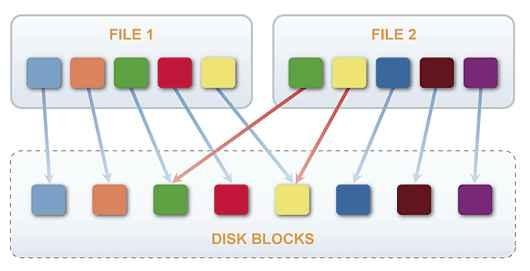
\includegraphics[width=10cm]{img/deduplication.jpg}

Il existe deux types de dépuplication: la déduplication à la volée (à la source) et la déduplication hors ligne (à la destination). La déduplication à la volée analyse les fichiers avant de les stocker pour savoir s'ils n'existent pas déjà sur le disque. Cette technique utilise une forte consommation CPU et mémoire. L'autre technique consiste à copier dans un premier temps le fichier sur le disque avant de tester s'il existe déjà. Cela nécessite de prévoir un espace de stockage tampon plus important. \\

Dans un contexte de serveur de messagerie et de fichiers centralisés, la déduplication de données peut très rapidement économiser de nombreux gigaoctets d'espace disque ainsi que la diminution de la bande passante qui aurait été utilisée pour la sauvegarde. En effet, dans le cas où un même mail de 1Mo est envoyé à cinquante destinataires alors l'économie du disque sera de 50-1 megaoctets (stockage d'un seul mail). La déduplication est faite pour des fichiers tels que des documents bureautiques ou des machines virtuelles qui ont souvent de nombreux blocs en commun.\\
Le terme inverse de la déduplication est la réhydratation. Elle fait appel à la table des index afin de renvoyer tous les blocs de données référencés pour un fichier demandé.\\

Certain outils comme LessFS mise en relation avec un système de fichiers ZFS permettent de dédupliquer et de compresser les blocs de données. Cela permet de gagner encore plus d'octets sur le disque mais nécessite une consommation mémoire et CPU plus importante.

	\subsection{ZFS}
	\subsubsection{Introduction}
	Le système de fichier ZFS (Zettabyte File System) a été conçu par Sun en 2005 et est sous licence CDDL.  Il n'était disponible que sous Solaris mais est devenu récemment disponible sous linux. Il est l'un des systèmes de fichiers les plus intéressants du marché. En effet, ZFS intègre de nombreux avantages que d'autres n'ont pas. Voici une liste de ses principaux avantages: \\
	\begin{itemize}
		 \item Pas de limite pratique (taille des disques, fichiers, ...)
		 \item Garantir la sécurité des données (intégrité, disponibilité)
		 \item Administration simplifiée
		 \item Gestionnaire de volume intégré
		 \item Compression
		 \item Snapshot
		 \item Duplication
		 \item Quotas et réservation d’espace
		 \item Performances élevées
		 \item Indépendant de l’architecture matérielle\\
	\end{itemize}
	ZFS est un système de fichier 128 bits contrairement aux autres systèmes qui sont de 64 bits. Ainsi ses limites sont de 16 milliards de milliards fois plus, autant dire qu'il n'a quasi pas de limite. Afin d'optimiser ses performances, ZFS utilise tout l'espace disponible de la RAM pour créer un énorme cache. Ce procédé s'appelle ARC (Adaptive replacement cache). Il peut poser problème aux autres processus qui testent la mémoire inutilisée avant de ce lancer mais cette mémoire est souvent inutilisée. Il peut être partagé via le réseau avec d'autres systèmes de fichiers comme nfs ou samba. Ainsi même depuis des systèmes qui ne le supporte pas, il sera accessible.\\
	\subsubsection{Stockage}
	ZFS fonctionne avec un pool. C'est un ensemble de périphériques qui fournissent de l’espace pour le stockage et la duplication des données comme le raid logiciel. \\
	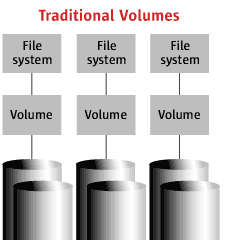
\includegraphics[width=5cm]{img/volumes_tradicionais.png}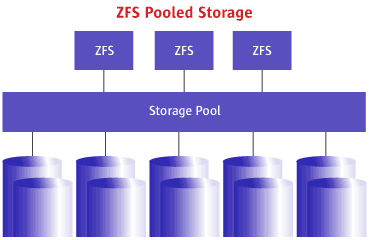
\includegraphics[width=7cm]{img/armazenamento_pooled_zfs.png}\\
	Voici les différentes unités de base de stockage de données :\\
	\begin{itemize}
		 \item Disques : entiers ou juste une partition
		 \item Fichiers dans un autre système de fichiers
		 \item Miroirs : 2 (ou plus) disques, partitions ou fichiers
		 \item Raid-z : plusieurs disques, variante de RAID-5\\
	\end{itemize}
	ZMirror est un miroir classique. Il utilise les mécanismes de checksum pour valider les lectures sur un composant et bascule sur le second s'il détecte une erreur puis corrige le composant défaillant (si possible). Le système Raid-z est similaire au procédé Raid 5. Il utilise les checksums (SHA-256 + fletcher) et repose sur le copy on write : supprime le "write-hole".
	\subsection{Compression}
	Tout comme la déduplication, la compression est une technique qui permet d'économiser de l'espace de stockage. Chaque fichier est constitué d'une succession de millions de bits 0 ou 1. La compression permet de diminuer le nombre de bits que constitue un fichier en changeant la succession de bits de départ. Suivant l'algorithme de codage utilisé, le taux de compression peut différer. Les algorithmes d'encodage sont plus ou moins efficaces selon le type de fichier compressé.\\
 Il existe deux types de compression: la compression avec perte et sans perte. La compression sans perte signifie qu'après la décompression, le fichier sera identique au fichier compressé. C'est le plus souvent utilisé sur des documents, des fichiers exécutables ou des archives. Ces données étant principalement des caractères texte, ils ne peuvent pas être modifiés. Les formats de documentation tels que txt, doc ou pdf sont donc compressés sans perte.  Par contre, lors d'une compression avec perte, les fichiers décompressés ne seront pas exactement identiques au fichier original mais les informations seront sensiblement les mêmes. Les types de fichiers utilisés par cette compression sont les images, les sons et les vidéos. Cett technique se repose sur la limitation des sens de l'homme comme la vision et l'audition. L'homme ne pourra donc pas identifier les différences entre le fichier original et le fichier après décompressage. Les formats de fichiers jpeg, avi ou mp3 sont donc compressés avec pertes. \\
Pour chaque technique de compression, il existe plusieurs algorithmes de codage.\\
	\subsubsection{Compression sans perte}
		Parmi les algorithmes sans perte, il y a les algorithmes tels que Lempei-Ziv ou le codage RLE (Run-Length Encoding) qui consistent à remplacer des suites de bits utilisées plusieurs fois dans un même fichier. D'autres algorithmes comme l'algorithme de codage Huffman détermine les suites de bits et plus une suite est utilisée souvent, plus la suite qui la replacera sera courte. 
Voici les différents types de compression sans perte:
		\begin{itemize}
			\item L'algorithme Lempel-Ziv
			\begin{itemize}
				\item LZ77	
				\item LZ78
				\item LZO
			\end{itemize}
			\item L'algorithme RLE
			\item Codage par modélisation de contexte
			\begin{itemize}
				\item Prédiction par reconnaissance partielle (PPM)
				\item Pondération de contextes (CM)
			\end{itemize}
			\item L'algorithme de codage Huffman
		\end{itemize}
	\subsubsection{Compression avec pertes}
		La compression avec pertes s'utilisent donc sur des données perceptibles par l'homme comme les sons, les images ou les vidéos. Elle supprime les données que l'homme ne perçoit pas ou quasiment pas. Ainsi pour le format JPEG 2000, la compression est de 1 bit/pixels au lieu de 24 bits/pixels. La compression avec pertes est une technique irréversible c'est à dire qu'il ne sera pas possible de retrouver le fichier original. Il existe trois grandes familles de compression avec pertes: la compression par prédiction, par transformation et la compression basée sur les récurrences fractales de motif.\\
 Voici les différents types de compression avec pertes:
		\begin{itemize}
			\item Compression par prédiction
			\item Compression par transformation
			\item La norme JPEG
			\item Compression par ondelette
			\item Compression basée sur les récurrences fractales de motif
		\end{itemize}

\section{Logiciels}


\subsection{Areca Backup}
\subsubsection{Caractéristiques}
\begin{itemize}
  \item Archives de compression en format Zip et Zip64.
  \item Archives de cryptage (AES128 et algorithmes de chiffrement AES 256).
  \item Stockage sur disque dur local, lecteur réseau, clé USB, FTP, FTPS (implicite et explicite avec SSL / TLS) ou un serveur SFTP.
  \item Filtres de fichier : par extension, répertoire, expression régulière, taille, date, statut, avec AND / OR /NOT logique.
  \item Sauvegarde Incrémentielle, différentielle et sauvegarde complète.
  \item Archives et fusions : Permet fusionner les archives contigus dans une archive unique pour économiser l'espace de stockage.
  \item Sauvegarde à partir d'une date donnée : Permet de récupérer des archives à partir d'une date spécifique.
  \item Mécanisme de transaction : tous les processus critiques, telles que les sauvegardes ou fusions sont transactionnels (commit rollback). Cela garantit l'intégrité des sauvegardes.
  \item Rapports de sauvegarde : Areca génère des rapports de sauvegarde qui peuvent être envoyés par email.
  \item Progammation de scripts de sauvegarde : Areca peut lancer des scripts shell après la sauvegarde.
  \item Les permissions des fichiers, liens symboliques et les pipes nommés peuvent être stockés et récupérés (Linux uniquement).
  \item Les tâches: Une tâche de sauvegarde est appelée «target» dans la terminologie de Areca. Il définit les fichiers qui seront stockés (sources), où ils seront stockés (destination) la façon dont ils seront stockés (si elles seront compressées, cryptées, etc.).
Les «targets» peuvent être organisés en «targets groups».
  \item Areca utilise la taille du fichier et date de dernière modification pour détecter les fichiers modifiés, si un de ces attributs est modifié (quelle que soit sa valeur), le fichier est marqué comme modifié. Cela permet une détection rapide des fichiers modifiés.

\end{itemize}

\subsubsection {Modes de stockage}
Areca peut gérer de multiples modes de stockage:
\begin{itemize}
  \item Standard: C'est le mode par défaut, une nouvelle archive sera créée pour chaque sauvegarde. Tous les fichiers nouveaux ou modifiés depuis la dernière sauvegarde seront stockés dans cette archive.
  \item Delta: Une nouvelle archive sera créée pour chaque sauvegarde. Tous les *parties* modifiées de fichiers depuis la dernière sauvegarde seront stockés dans cette archive. Ce mode est particulièrement utile pour la manipulation des fichiers volumineux. (Areca utilise un algorithme qui est similaire à rsync pour détecter et gérer les parties modifiées des fichiers).
  \item Image: Une archive unique sera créé et mis à jour à chaque sauvegarde.
\end{itemize}

\subsubsection {types de sauvegarde}
Areca peut gérer les types de sauvegardes suivants:
\begin{itemize}
  \item Sauvegarde complète: Lors d'une sauvegarde complète est effectuée, tous les fichiers sont stockés dans une archive (même s'ils ont été modifiées ou non).
  \item Sauvegarde incrémentale: Quand une sauvegarde incrémentale est réalisée, seuls les fichiers qui ont été modifiés depuis la dernière sauvegarde sont stockés dans l'archive.
  \item La sauvegarde différentielle: Lors d'une sauvegarde differentiel est effectuée, seuls les fichiers qui ont été modifiés depuis la dernière sauvegarde complète sont stockés dans l'archive.
\end{itemize}

\subsection{Bacula}
Bacula est un ensemble de programmes qui permet de gérer des sauvegardes, restaurations ou vérifications de données d'un ordinateur sur un réseau hétérogène.
\subsubsection{Caractéristiques}
\begin{itemize}
  \item Il utilise une base de données relationnelle motorisée par MySQL, PostgreSQL ou SQLite.
  \item Crée des signatures SHA-1 (ou MD5) pour chaque fichier sauvegardé.
  \item Permet le chiffrement des données et des commandes transitant sur le réseau et peut sauvegarder des fichiers de plus de 2 Go.
  \item Capable de gérer les robots changeurs de bandes.
  \item Peut exécuter des scripts avant et après de chaque travail.
\end{itemize}

\subsubsection{Services de Bacula}
\begin{itemize}
  \item Le service \textbf{Bacula Director} est le programme qui supervise toutes les opérations de sauvegarde, restauration, vérification et archivage. L'administrateur système utilise le Bacula Director pour planifier les sauvegardes et restaurer les fichiers.
  \item Le service \textbf{Bacula Console} est le programme qui permet à l'administrateur ou à l'utilisateur de communiquer avec le Bacula Director. Actuellement, le service Bacula Console est disponible en trois versions. La première et la plus simple est d'exécuter le programme Console dans une fenêtre shell (i.e. interface TTY). La seconde version est une interface graphique GNOME. La troisième version est une interface graphique wxWidgets qui permet de sélectionner interactivement les fichiers à restaurer. Elle intègre la plupart des fonctionnalités de la console shell, permet la complétion automatique avec la touche tabulation, et fournit une aide instantanée relative à la commande tapée.
  \item Le service \textbf{Bacula File} (ou programme client) est le programme installé sur la machine à sauvegarder. Il est spécifique au système sur lequel il est exécuté et a la charge de fournir les attributs des fichiers et les données requis par le Director. Les Services File sont aussi chargés de la partie dépendant du système de fichiers lors de la restauration des attributs de fichiers et des données. Ce programme est exécuté en tant que service sur la machine à sauvegarder. En plus du File Daemon pour Unix/Linux, il existe un File Daemon pour Windows (usuellement distribué au format binaire). Le File Daemon Windows fonctionne sur toutes les versions actuelles de Windows (NT, 2000, XP, 2003 et peut-être aussi 98 et Me).
  \item Le service \textbf{Bacula Storage} est le programme qui transfère les données et les attributs de fichiers aux média physiques ou aux volumes et les restitue lors de restaurations. En d'autres termes, Le storage Daemon est responsable des opérations de lecture et d'écriture sur les cartouches (ou autres média de stockage, comme par exemple des fichiers).
  \item Les services \textbf{Catalogue} ont pour tâche de maintenir à jour la base de données des index de fichiers et volumes pour tous les fichiers sauvegardés. Les services Catalogue permettent à l'administrateur système ou à l'utilisateur de localiser rapidement et restaurer n'importe quel fichier. Les services Catalogue de Bacula le placent dans une catégorie différente de programmes tels que tar et bru, puisque le catalogue Bacula maintient un enregistrement de chaque volume utilisé, chaque job exécuté et chaque fichier sauvegardé ce qui permet des restaurations et une gestion de volumes efficaces.
\end{itemize}


\subsection{Amanda}
\subsubsection{Caractéristiques}
\begin{itemize}
  \item Il est basé sur des outils standards (dump, restore, tar, etc.).
  \item Son architecture modulaire répartit, les tâches sur des machines périphériques.
  \item Architecture un client/serveur : Permet la possibilité de réaliser des copies de systèmes physiquement éloignés mais branchés sur le même réseau et génère un environnement facilement escalable.
  \item Une Sécurité : Les communications peuvent être protégés en utilisant OpenSSH ou des algorithmes de chiffré.
  \item Cache dans un disque : Amanda stocke les copies dans un disque pour éviter des pertes de données et pour améliorer la vitesse d'enregistrement.
  \item Il implémente une gestion des bandes simple et efficace : on ne peut effacer une bande par erreur, et il existe des outils de recherche de fichier dans toute la collection de support.
  \item Interface générique des changeurs de bandes, donc, non seulement on peut utiliser des dérouleurs différents, mais aussi des robots différents.
  \item Ajuste l’ordonnancement par des règles d’optimisation.
  \item Intégre des outils de rapport, hautement configurables et modifiables.
  \item Autorise l’inclusion de tout module que l’on désire.
  \item Peut encrypter ou compresser tant les communications avec les agents de sauvegarde, que les supports eux-mêmes.
\end{itemize}

\chapter{Conclusion}

\paragraph{}
Après avoir effectué un nombre considérable de recherches bibliographiques sur la sauvegarde en général, les techniques d'optimisation de ces programmes, et les logiciels permettant la mise en oeuvre de sauvegardes, il s'agira maintenant de tester les différents logiciels de sauvegarde.
Pour cela, il faudra mettre en place une infrastructure qui nous permettra de réaliser ces tests sur une échelle réelle.

\paragraph{}
La plateforme de tests devra nous permettre d'effectuer différents tests, et ce dans différentes situations d'utilisation.
Les différents scénarios d'utilisation qui sont envisagés seront une base de données, un serveur mail, un serveur de fichiers, et des machines virtuelles.

\paragraph{}
Différentes méthodes de sauvegardes seront aussi envisagées, tel que des sauvegardes complètes, des sauvegardes continues, des snapshots, et des sauvegardes hors-site.

\paragraph{}
Nous réfléchirons aussi à l'impact de ces sauvegardes dans le cas de différents incidents.
En effet, il faudra analyser et comprendre l'efficacité de ces sauvegardes dans le cas d'un fichier malencontreusement effacé ou corrompu, d'un système hors service et dont les données sont irrécupérables, ou encore une catastrophe majeure qui impacterait l'ensemble du site tel qu'un feu ou une innondation.

\paragraph{}
Il serait interessant de se pencher sur la délégation de tâches pour les utilisateurs, aussi bien au niveau de la sauvegarde que de la restauration.
En effet, les utilisateurs ont tendance à vouloir effectuer eux-même ces opérations, surtout quand il s'agit de mauvaises manipulations de leur part.

\paragraph{}
Comme one l'a vu, la sauvegarde en elle-même n'est pas une solution complète mais fait partie d'un mécanisme permettant d'assurer l'intégrité des données.
Aussi, on s'interressera aux concepts qui font partie de ce mécanisme, tel que les plans de reprise d'activité.
L'élaboration de ces plans est tout aussi importante que la création d'une stratégie de sauvegarde, car elle indiquera clairement la marche à suivre en fonction des différents évènements, et permettront de gagner un temps précieux.

\paragraph{}
On s'interressera aussi plus longuement sur les types de sauvegardes à adopter dans un contexte de machines virtuelles.
En effet, avec l'augmentation croissante des machines virtuelles, réaliser la sauvegarde de celles-ci alors qu'elles sont en cours d'utilisation peut devenir un vrai casse-tête.



%\begin{abstract}
%\end{abstract}

\end{document}          
